\section{Saturn's two Moons}
In order to solve the problem of the orbit shift, the Stoerms method is used.
The equations feed to the library are seen in equation \ref{eq:equations_saturn}.

\begin{equation}
\large{
\begin{array}{ll}
\frac{d^2x_1}{dt^2} = - \frac{M g x_1}{r_1^3} + \frac{m_2 g (x_2 - x_1)}{r_{12}^3} &
\frac{d^2y_1}{dt^2} = - \frac{M g y_1}{r_1^3} + \frac{m_2 g (y_2 - y_1)}{r_{12}^3}\\
\frac{d^2x_2}{dt^2} = - \frac{M g x_2}{r_2^3} - \frac{m_1 g (x_2 - x_1)}{r_{12}^3} &
\frac{d^2y_2}{dt^2} = - \frac{M g x_2}{r_2^3} - \frac{m_1 g (y_2 - y_1)}{r_{12}^3}
\end{array}
}
\label{eq:equations_saturn}
\end{equation}

The maximum error is calculated with the StepperStoerm algorithm in NR.
Using that the number of iterations is counted to 3412. The worst case error is 10.236 km.
The distance from the moon to Saturn can be seen in figure \ref{fig:distance}.
The crossing point happens about 130 and 530 days.

The phase difference between the two moons is at it's lowest when the moons swap orbit as seen in figure \ref{fig:angle}.

\begin{figure}[h]
\centering
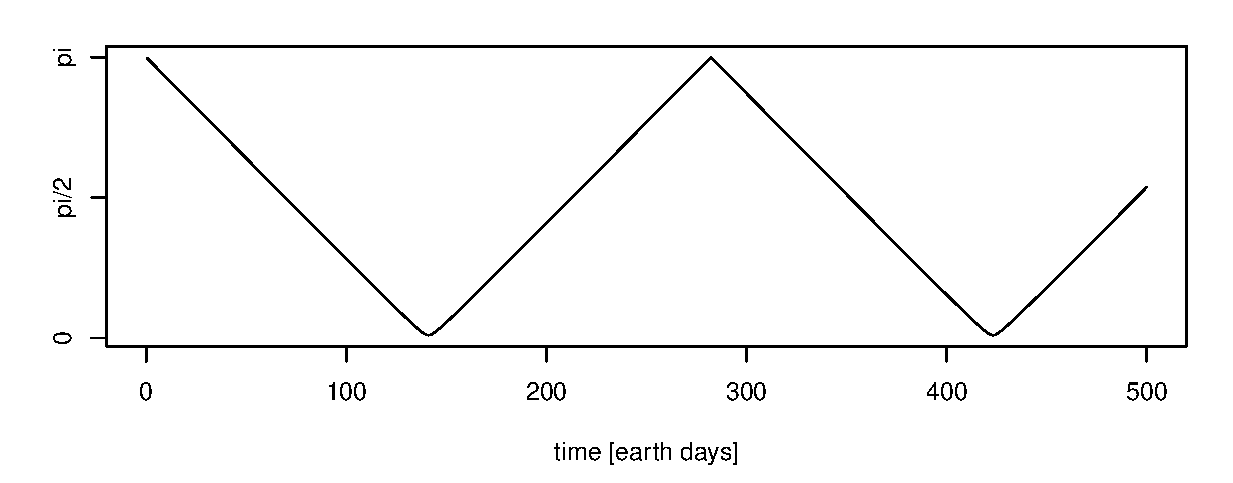
\includegraphics[width=0.9\textwidth]{graphics/angle}
\caption{Absolute phase difference between the two moons.}
\label{fig:angle}
\end{figure}

\begin{figure}[h]
   \centering
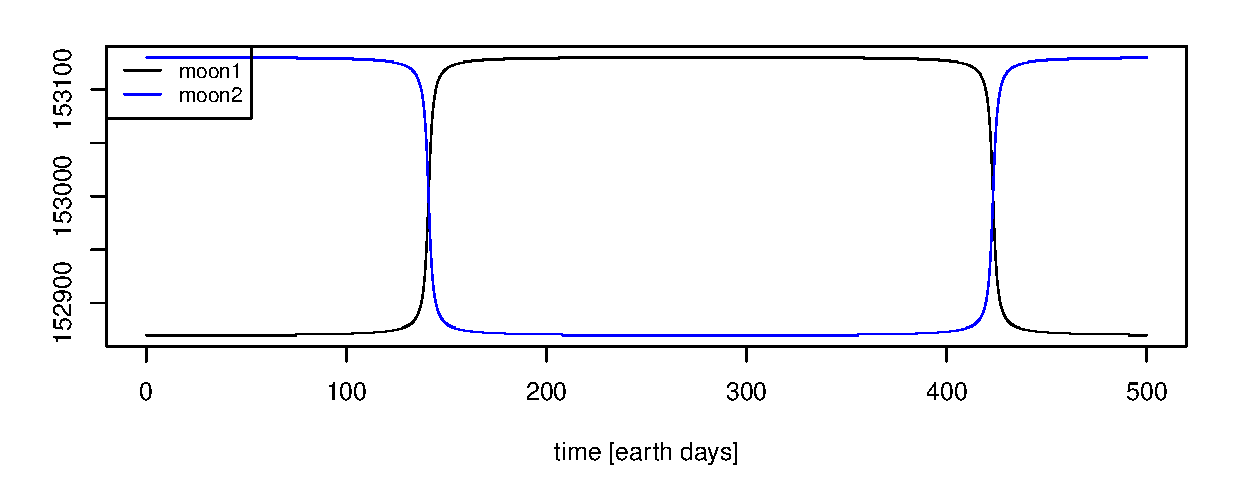
\includegraphics[width=0.9\textwidth]{graphics/distance}
\caption{Distance from the moons to Saturn}
\label{fig:distance}
\end{figure}



